\documentclass[a4paper]{article}

\usepackage[english]{babel}
\usepackage[utf8]{inputenc}
\usepackage{amsmath}
\usepackage{graphicx}
\usepackage[colorinlistoftodos]{todonotes}
\usepackage[left=2cm, right=2cm, top=2cm]{geometry} 
\usepackage{float}
\title{Turning Delta Function into Continuous}

%\author{Your names and group number}

\date{\today}

\begin{document}
\maketitle

\begin{abstract}
This is an attempt to try and describe how modeling the delta function as a continuous function. Right now I'm considering an extremely simple situation, where I just have a flat region with a single delta function. I approximate this delta function as a triangle, and I'm trying to figure out how the width of this triangle affects its accuracy.
\end{abstract}



\section{Run \#1}\label{sec:run1}
\subsection{Generating phonon distributions}
I generated the pretend phonon distributions using the ``generateInput.py'' code, that exists in the ``run1'' directory. This created a series of 5 fake frequency distributions, shown in Fig.~\ref{fig:run1}. These distributions are generated between 0 and 1, with a spacing of 0.01. The delta function is to be located at 0.5, and the area of the delta function is to be held at 0.2, while the area of the continuous piece (the flat piece) is to be held at 1.0. The thinnest triangle (blue) has a base width of $(2\times0.01)=0.02$, while the largest one (purple) has a base width of $(10\times0.01)=0.1$.

\begin{figure}[H]
\centering
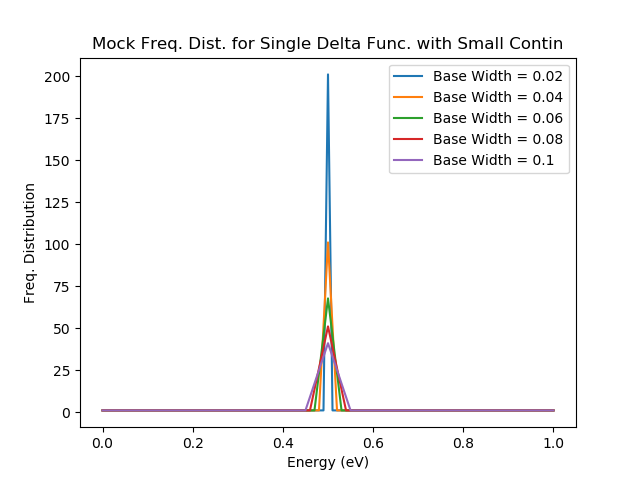
\includegraphics[width=0.8\textwidth]{phononDist_run1}
\caption{\label{fig:run1}Fake frequency distributions of Run \#1~mentioned in Sec.\ref{sec:run1}. For this I consider five different continuous representations of a delta function, each a triangle with varying width. The delta function is normalized to have an area of 0.2, the flat region has an area of 1.0. The delta function is centered at 0.5, and the grid has a spacing of 0.01.}
\end{figure}


\subsection{Running with Delta Funcs. vs. with Triangle-Approximated Delta Funcs.}
\begin{figure}[H]
\centering
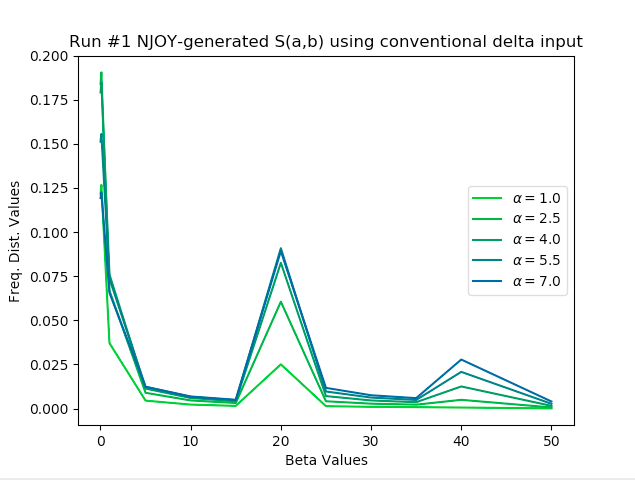
\includegraphics[width=0.6\textwidth]{run1_sab_using_just_delta_funcs.png}
\caption{\label{fig:run2_just_delta} The $S(\alpha,\beta)$ results are shown above, after running the simple, single delta function input, using delta functions instead of triangle-approximated delta functions.}
\end{figure}


\newpage


\section{Run \#2}
\subsection{Generating phonon distributions}
I generated the pretend phonon distributions using the ``generateInput.py'' code in the ``run2'' directory. This is meant to create something close to the H in H2O model used in the NJOY test, with approximated delta functions included in the higher energy region.\par
The low energy distribution was copied from Test 09 of the NJOY 2016 release. This is also where I got the locations and weights for the delta functions. The lower delta function is centered at 0.205 eV, with a weighting of 0.16667, while the higher one is centered at 0.48 eV with a weighting of 0.33333. The continuous piece (which is only nonzero at the low energy region) has a weighting of 0.4444. The spacing used for this run is 0.005, which differs from the 0.00255 used in the Test 09 example. The resultant frequency distribution is shown in Fig.~\ref{fig:run2}.\par

\begin{figure}[H]
\centering
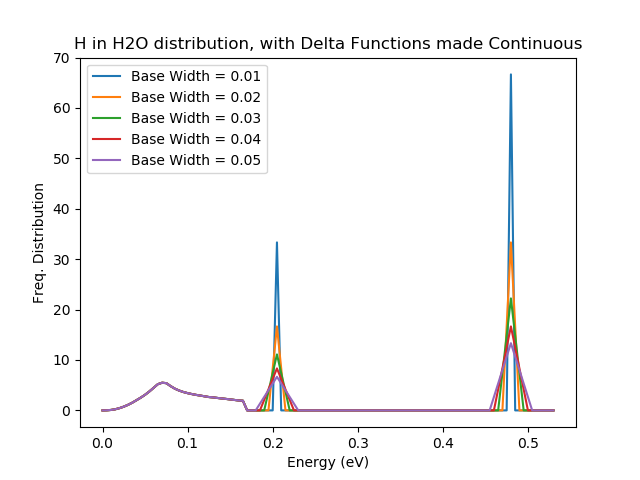
\includegraphics[width=0.8\textwidth]{phononDist_run2}
\caption{\label{fig:run2}The generated phonon distribution for run \#2 is shown here. This Is meant to strongly resemble the H in H$_2$O input, where the low-energy continuous distribution and its weight is taken from NJOY2016 Test09, along with the positions/weights of the delta functions. }
\end{figure}



\subsection{Running with Delta Funcs. vs. with Triangle-Approximated Delta Funcs.}
I used NJOY to run the 6 relevant cases: H in H2O with (1) delta functions approximating the higher energy peaks, and with (2-6) triangles of base width 0.002, 0.004, 0.006, 0.008, and 0.010. These input files are saved in the directory ``run2'' under the names ``yDelta'' and ``nDelta\_triangleWidthX\_run2'' for $X=2,4,6,8,10$.\par
Fig~\ref{fig:run2_just_delta} shows the $S(\alpha,\beta)$ produced by using the conventional $\delta$-function input, plotted against $\beta$ for various $\alpha$. Note that there is extremely high variation between the $S(\alpha,\beta)$ values for various $\alpha$ and $\beta$.\par
\begin{figure}[H]
\centering
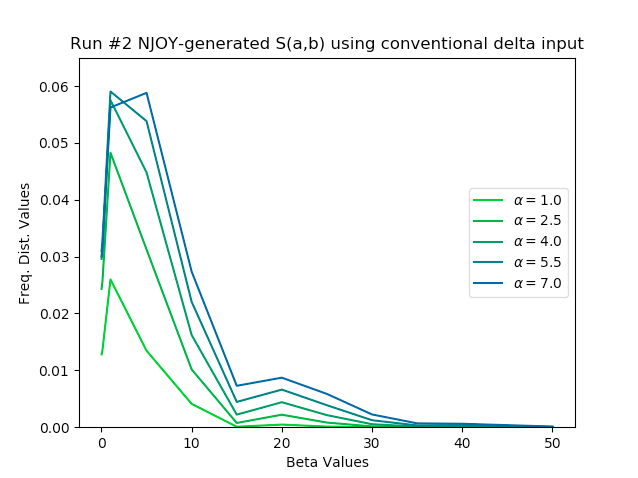
\includegraphics[width=0.6\textwidth]{run2_sab_using_just_delta_funcs.png}
\caption{\label{fig:run2_just_delta} The $S(\alpha,\beta)$ results are shown above, after running the H in H$_2$O input using delta function inputs. Note that the resultant $S(\alpha,\beta)$ distribution is highly variant on input $\alpha,\beta$ values. Keep the scale in mind when we look at the absolute difference between with delta functions vs. without delta functions, for the later graphs.}
\end{figure}

Fig.~\ref{fig:run2_comparing_sab_values} shows the results of $S(\alpha,\beta)$, comparing the ``true'' $\delta$ function result, vs. the triangle-approximated results, with three separate plots depicting $\alpha=1.0,4.0,$ and 7.0.

\begin{figure}
\centering
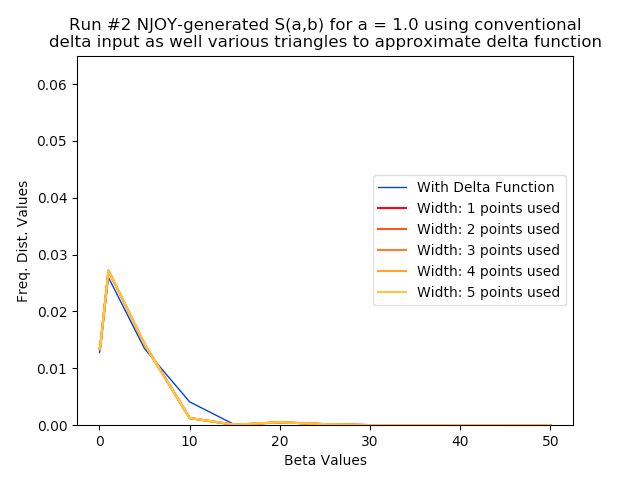
\includegraphics[width=0.49\textwidth]{run2_sab_alpha_equals_1.png}
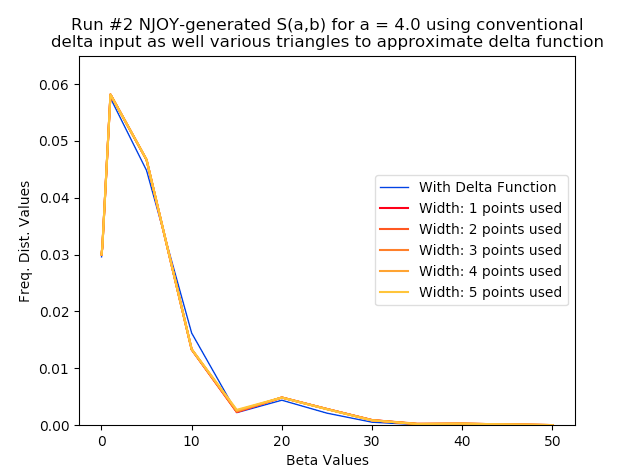
\includegraphics[width=0.49\textwidth]{run2_sab_alpha_equals_4.png}
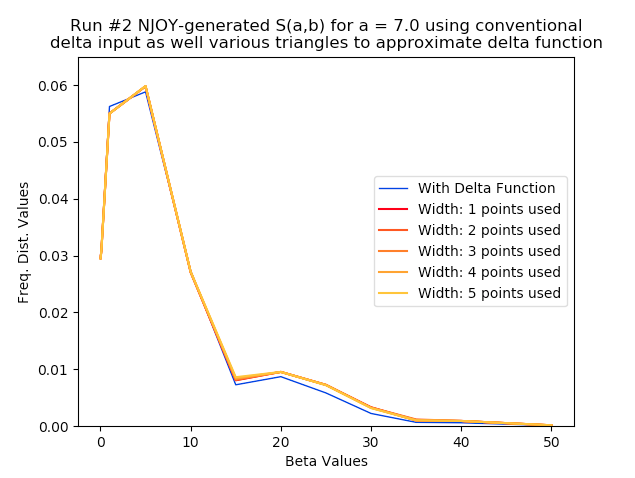
\includegraphics[width=0.49\textwidth]{run2_sab_alpha_equals_7.png}
\caption{\label{fig:run2_comparing_sab_values} The $S(\alpha,\beta)$ results are shown above, after running the H in H$_2$O input using both delta function inputs and triangle-approximated inputs. This is run for $\alpha=$1.0,4.0, and 7.0 separately. Note that the approximated $S(\alpha,\beta)$ follows the delta-function $S(\alpha,\beta)$ very well, and that the various widths of triangles does not seem to have a significant effect on the resultant $S(\alpha,\beta)$.}
\end{figure}
























































%\section{Intro}
%\label{sec:introduction}
%\cite{nano3}.

%\section{Theory 2-3 pages}
%\label{sec:theory}

%\subsection{Two-dimensional Electron Gas}

%\subsection{Quantum Hall Effect}

%\begin{figure}
%\centering
%\includegraphics[width=1\textwidth]{raw_data.png}
%\caption{\label{fig:data}Raw (unprocessed) data. Replace this figure with the one you've made, that shows the resistivity.}
%\end{figure}
%

%\newpage
%\begin{figure}
%\centering
%\includegraphics[width=0.3\textwidth]{frog.jpg}
%\caption{\label{fig:frog}this frog was uploaded to writelatex via the project menu.}
%\end{figure}


%\begin{table}
%\centering
%\begin{tabular}{l|r}
%Item & Quantity \\\hline
%Widgets & 42 \\
%Gadgets & 13
%\end{tabular}
%\caption{\label{tab:widgets}An example table.}
%\end{table}

%\begin{equation}
%S_n = \frac{X_1 + X_2 + \cdots + X_n}{n}
%      = \frac{1}{n}\sum_{i}^{n} X_i
%\label{eq:sn}
%\end{equation}
%
%denote their mean. Then as $n$ approaches infinity, the random variables $\sqrt{n}(S_n - \mu)$ converge in distribution to a normal $\mathcal{N}(0, \sigma^2)$.

%The equation \ref{eq:sn} is very nice.


%\subsection{How to Make Lists}

%You can make lists with automatic numbering \dots

%\begin{enumerate}
%\item Like this,
%\item and like this.
%\end{enumerate}
%\dots or bullet points \dots
%\begin{itemize}
%\item Like this,
%\item and like this.
%\end{itemize}
%\dots or with words and descriptions \dots
%\begin{description}
%\item[Word] Definition
%\item[Concept] Explanation
%\item[Idea] Text
%\end{description}


%\begin{thebibliography}{9}
%\bibitem{nano3}
%  K. Grove-Rasmussen og Jesper Nygård,
%  \emph{Kvantefænomener i Nanosystemer}.
%  Niels Bohr Institute \& Nano-Science Center, Københavns Universitet
%
%\end{thebibliography}


\end{document}
